\section{Používateľská špecifikácia} % 3-4 strany
\subsection{Stručný úvod do problematiky}

\acrfull{mhs} \projectName\ má ľuďom uľahčiť vyhľadávanie a rezerváciu 
ubytovania v rôznych krajinách sveta.
Systém je určený pre dve skupiny používateľov. 
Pre potenciálnych zákazníkov hotelov alebo iných ubytovacích zariadení, 
ktorí si chcú rezervovať najviac vyhovujúce ubytovanie v čo najlacnejšej 
ponuke v ich vybranej lokalite v určitom čase. 
A pre poskytovateľov ubytovania, ktorí dokážu a chcú poskytovať ubytovanie 
a služby s tým spojené. 
\acrshort{mhs} eviduje všetky možné destinácie, v ktorých si vie 
potenciálny zákazník vyberať a porovnávať ubytovacie zariadenia a následne 
zarezervovať vo vybranom čase, ak je ubytovacie zariadenie vtedy voľné. 
Evidenciu destinácií vytvárajú samotní poskytovatelia ubytovancích zariadení, 
pri zadávaní lokalít, kde sa nachádza poskytované ubytovanie. 
Poskytovatelia ubytovania môžu byť fyzické osoby, živnostníci, hotely, 
cestovné kancelárie a rôzne iné spoločnosti, ktoré sa zaoberajú turizmom 
a hotelierstvom. 
Po zaregistrovaní poskytovateľa ubytovania v \acrshort{mhs} a overení 
pravdivosti údajov je mu vytvorený účet v systéme, do ktorého môže vložiť 
svoju ponuku ubytovania a k nemu prezentačné materiály o ubytovaní a 
informácie ako repertoár poskytovaných služieb, cenník, počet voľných 
miest v rôznych časových obdobiach, kontaktné údaje, podmienky a 
pravidlá ubytovania a poprípade zaujímavé tipy na výlety, občerstvenie 
alebo aktivity. Neregistrovaný poskytovateľ nie je schopný vykonať takéto 
úkony v \acrshort{mhs}, kvôli ochrane potenciálneho zákazníka, aby mal 
istotu, že poskytovateľ je skutočná osoba alebo subjekt a ubytovacie 
zariadenie vôbec existuje alebo existuje na danom mieste a vedia mu 
garantovať všetko, čo by bolo v ponuke ubytovania uvádzané a nebol teda 
zákazník zavádzaný. Potenciálny alebo už aktuálny zákazník registráciou 
do \acrshort{mhs} vie získať možnosť hodnotiť ubytovacie zariadenia ako 
aj ich poskytovateľov a nimi ponúkané služby a to aj anonymne a taktiež 
mu \acrshort{mhs} vie uložiť a poskytnúť k nahliadnutiu celú históriu 
rezervácii ubytovaní. Neregistrovaní zákazníci vedia iba vyhľadávať a 
prezerať si všetky ponuky ubytovania v rôznych krajinách sveta.
Na samotnú rezerváciu ubytovania musí zákazník byť registrovaný a to z 
dôvodu ochrany poskytovateľov ubytovania, aby zákazník bol viazaný na 
určité pravidlá a povinosti pri rezervovaní ubytovania a aby poskytovateľ 
mal zaručený kontakt so zákazníkom, pri vzniknutých komplikáciach z 
poskytovateľovej strany. \acrshort{mhs} poskytuje podporu pre automatické 
zisťovanie rôznych parametrov prostredníctvom webových služieb alebo ako 
\acrfull{api}, ktoré zabezpečujú dostupnosť a aktuálnosť údajov v 
\acrshort{mhs}. Vďaka \acrshort{mhs} \projectName\ poskytovateľ nemusí mať 
na spravovanie rezervácií vyhradeného zamestnanca alebo skupinu personálu, 
keďže o veľkú časť sa postará už zákazník ako o samotnú rezerváciu 
izby/zariadenia v jeho určenom čase, vyplnenie a kontrolu správnosti údajov 
a oboznámenie sa so službami. Poskytovateľ už musí len zobrať na vedomie 
zákazníkovú rezerváciu, prijať ju alebo ju zamietnuť s relevantným dôvodom 
a kontaktovať s tým zákazníka. Pri prijatí rezervácie musí zabezpečiť 
personál, ak nejaký má, a zabezpečí sľúbené služby a čistotu priestorov 
pri príchode alebo počas celého pobytu zákazníka, podľa vopred dohodnutých 
podmienok.

\newpage

\subsection{Používateľské požiadavky}

\begin{enumerate}[label=\Alph*.]
    \item Funkcionálne požiadavky
    \begin{itemize}
        \item Vyhľadanie ubytovania
        \item Filtrovanie ubytovania podľa rôznych parametrov
        \item Prehliadanie ponuky ubytovania
        \item Prehliadanie informácií o ubytovaní
        \item Prehliadanie tipov od poskytovateľa pri ubytovaní
        \item Rezervácia ubytovania
        \item Platba za ubytovanie
        \item Zákazník nedokáže rezervovať ubytovanie bez registrácie
        \item Registrácia zákazníka
        \item Prihlásenie a odhlásenie zákazníka do jeho používateľského konta 
        pomocou mena a hesla
        \item Registrácia ubytovacieho zariadenia
        \item Poskytoytovateľ nedokáže registrovať ubytovanie bez 
        registrácie a overenia údajov
        \item Zadanie informácií k poskytovanému ubytovaniu
        \item Hodnotenie ubytovania alebo poskytovateľa
        \item Zákazník nedokáže hodnotiť ubytovanie alebo poskytovateľa 
        bez registrácie
        \item Hodnotenie zákazníka od poskytovateľa
        \item Poskytovateľ nedokáže hodnotiť ubytovaného zákazníka bez 
        registrácie
        \item Prehliadanie histórie rezervácií
        \item Prehliadanie pravidiel a povinností pri ubytovaní a 
        používaní systému
        \item Kontaktovanie poskytovateľa ubytovania
        \item Kontaktovanie zákazníka
    \end{itemize}
    \item Nefunkcionálne požiadavky
    \begin{itemize}
        \item Odlíšenie používateľského prostredia podľa typu zákazníka - 
        človek hľadajúci ubytovanie a poskytovateľ ubytovania
        \item Výsledky vyhľadávania sú zobrazené v akceptovateľnom čase
        \item Systém je kompatibilný so všetkými modernými operačnými
        systémamy
        \item Systém je kompatibilný so všetkými modernými webovými 
        prehliadačmi
        \item Systém je lokalizovaný v anglickom aj slovenskom jazyku
        \item Systém má prehľadné a moderné používateľské prostredie
        \item Overenie pravdivosti údajov pri registrácií poskytovateľa 
        ubytovania
        \item Využitie enkrypcie dát, pre znemožnenie botom vytvárať si 
        zákaznícke kontá a rezervovať si ubytovania
        \item Pri vyplnaní údajov do formulárov by malo byť dostatočne 
        vysvetlené, aké dáta sú požadované
        \item Systém poskytuje rôzne platobné metódy pri vykonávaní platby za 
        ubytovanie
    \end{itemize}
    \item Doménové požiadavky
    \begin{itemize}
        \item Systém dodržiava ochranu osobných údajov
        \item Určité údaje sú viditeľné len v rámci rezervačného kontraktu 
        pre poskytovateľa a zákazníka
        \item Poskytovateľove údaje sú ešte využité pre overenie informácií na 
        úradoch a v systémoch
    \end{itemize}
\end{enumerate}

%%%%%%%%%%%%%%%%%%%%%%%%%%%%%%%%%%%%%%%%%%%%%%%%%%%%%%%%%%%%%%%%%%%%%%%%

\section{Systémová špecifikácia}

\subsection{Diagramy prípadov použitia}

\begin{figure}[!htbp]
  \centering
  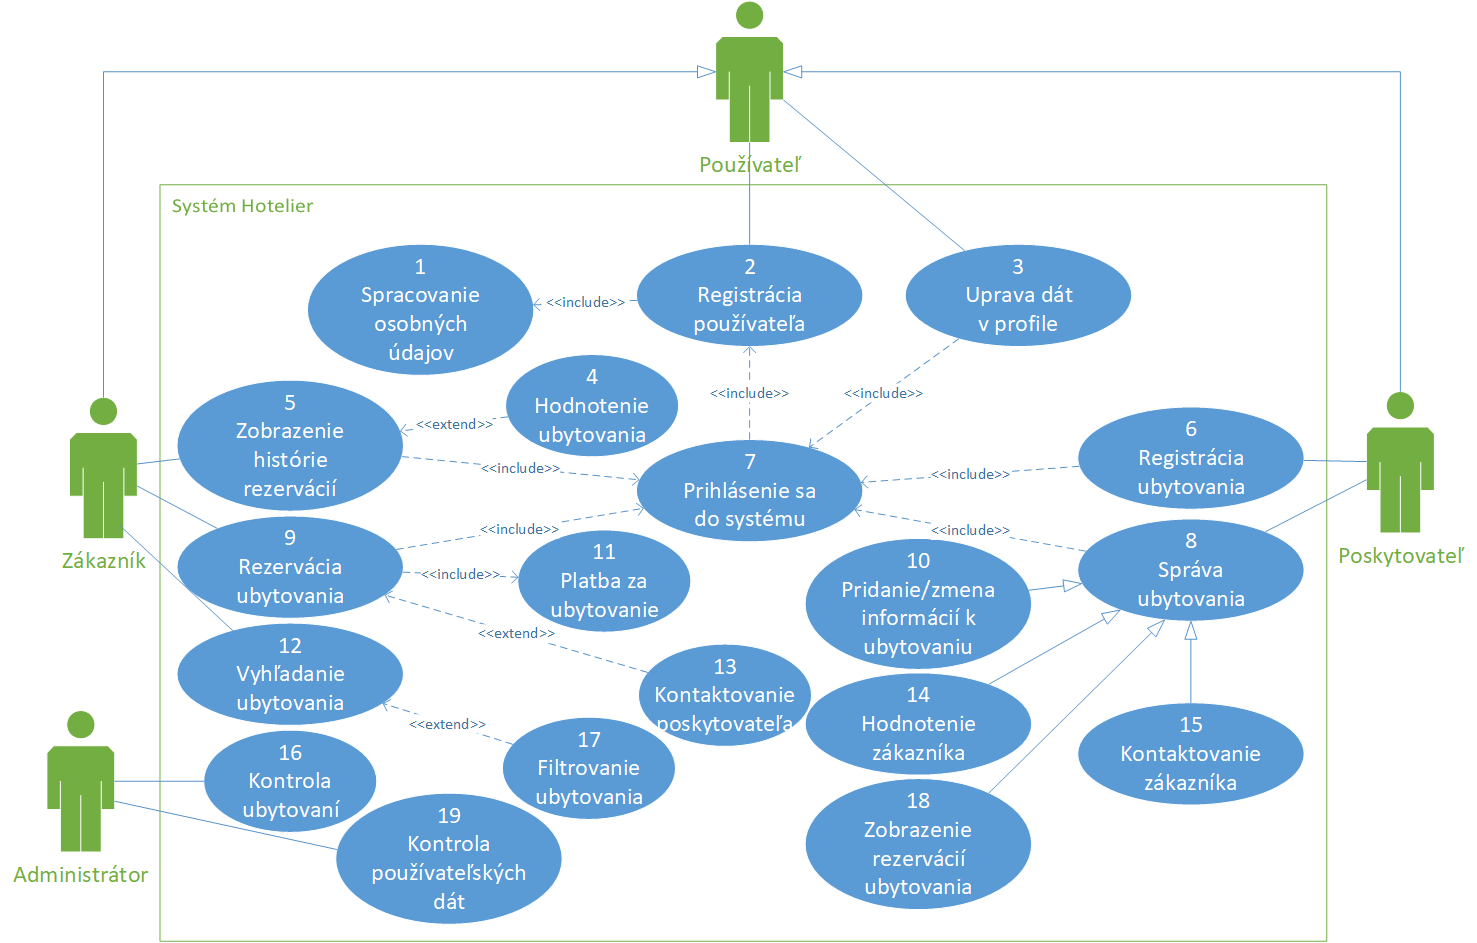
\includegraphics[width=\linewidth]{img/uc_diagram.png}
  \caption{Use case diagram}
  \label{uc_diagram}
\end{figure}	

\newpage

\subsection{Use-case tabuľky}

\begin{table}[h!]
    \centering
    \caption{Use case: Rezervácia ubytovania}
    \begin{tabular}{||p{\textwidth}||} 
        \hline
        \thead{Rezervácia ubytovania} \\ \hline\hline
        Číslo prípadu použitia: 9 \\ \hline
        Opis: Zákazník si rezervuje ubytovanie. \\ \hline
        Aktéri: Zákazník \\ \hline
        Vstupné podmienky: Zákazník je prihlásený. \\ \hline
        Inicializácia: Výber vyhľadaného ubytovania a stlačenie tlačidla 
        'Rezervovať'. \\ \hline
        Hlavný scenár:
            \begin{enumerate}
                \item Vyberie dátumy pobytu z voľných dátumov.
                \item Vyberie počeť osôb, ktorí sa chcú ubytovať, z povoleného 
                    počtu osôb.
                \item Vyberie spôsob platby plnej sumy.
                \item Skontroluje si rezervačné informácie.
                \item Prečíta si pravidlá a podmienky ubytovania a systému a 
                    potvrdí, že si ich prečítal.
                \item Zaplatí za rezerváciu.
            \end{enumerate} \\ \hline
        Alternatívny scenár 1:
            \begin{enumerate}[label=1.\arabic*]
                \item Ak zákazník nemá dostatok finančných prostriedkov pri 
                    vybranom spôsobe platby, po neúspešnej platbe ho systém 
                    upozorní a dovolí mu vybrať iný spôsob platby.
                \item Ak nechce pokračovať v platení, zruší rezerváciu tým, že 
                    odíde z rezervácie ubytovania.
            \end{enumerate} \\
        Alternatívny scenár 2:
            \begin{enumerate}[label=2.\arabic*]
                \item Zákazník môže zanechať správu poskytovateľovi pri 
                    rezervácii.
            \end{enumerate} \\ \hline
        Výstupné podmienky: Zákazník má rezevované ubytovanie. \\ \hline
    \end{tabular}
\end{table}

\newpage

\begin{table}[h!]
    \centering
    \caption{Use case: Vyhľadanie ubytovania}
    \begin{tabular}{||p{\textwidth}||} 
        \hline
        \thead{Vyhľadanie ubytovania} \\ \hline\hline
        Číslo prípadu použitia: 12 \\ \hline
        Opis: Zákazník si vyhľadá ubytovanie. \\ \hline
        Aktéri: Zákazník \\ \hline
        Vstupné podmienky: Zákazník sa nachádza na stránke systému. \\ \hline
        Inicializácia: Výber destinácie ubytovania. \\ \hline
        Hlavný scenár:
            \begin{enumerate}
                \item Zákazník vyberie mesto, kde by sa chcel ubytovať.
                \item Taktiež vyberie počet kilometrov od vybraného mesta, koľko 
                    je ochotný byť vzdialený od želaného mesta.
            \end{enumerate} \\ \hline
        Alternatívny scenár 1:
            \begin{enumerate}[label=1.\arabic*]
                \item Zákazník môže použiť filter na vyhľadanie ubytovania podľa 
                    jeho preferencií.
                \item Môže filtrovať mesto, kilometre od mesta, cenu, počet lôžok, 
                    služby (napr. bazén, výpožička bicyklov, atď.), pet-friendly, 
                    penzia, viac destinácií alebo aktivity v okolí ubytovania.
            \end{enumerate} \\ \hline
        Výstupné podmienky: Zákazník vyhľadal ubytovanie podľa jeho predstáv. \\ \hline
    \end{tabular}
\end{table}

\newpage

\begin{table}[h!]
    \centering
    \caption{Use case: Registrácia ubytovania}
    \begin{tabular}{||p{\textwidth}||} 
        \hline
        \thead{Registrácia ubytovania} \\ \hline\hline
        Číslo prípadu použitia: 6 \\ \hline
        Opis: Poskytovateľ registruje do systému svoje ponúkané ubytovanie. \\ \hline
        Aktéri: Poskytovateľ \\ \hline
        Vstupné podmienky: Poskytovateľ je prihlásený a overený. \\ \hline
        Inicializácia: Poskytovateľ stlačí tlačidlo v menu na zaregistrovanie 
        ubytovania. \\ \hline
        Hlavný scenár:
            \begin{enumerate}
                \item Poskytovateľ vyberie z evidovaných destinácií, kde sa jeho 
                    ubytovanie nachádza.
                \item Zadá adresu, kde je ubytovanie lokalizované.
                \item Zadá popis k ubytovaniu, fotky a cenu.
                \item Vyberie z uvedených parametrov, čo vie ubytovanie 
                    poskytovať ako napríklad počet lôžok, 
                    služby (napr. bazén, výpožička bicyklov, atď.), 
                    pet-friendly, penzia alebo aktivity v okolí ubytovania.
                \item Po stlačení tlačidla "Registrovať" sa záznam ubytovania 
                pošle systémovému administrátorovi na overenie. 
            \end{enumerate} \\ \hline
        Alternatívny scenár 1:
            \begin{enumerate}[label=1.\arabic*]
                \item Ak destinácia v systéme nie je evidovaná, poskytovateľ si 
                    ju vie zadať sám.
            \end{enumerate} \\ \hline
        Výstupné podmienky: Poskytovateľ má registrované ubytovanie. \\ \hline
    \end{tabular}
\end{table}

\newpage

\subsection{Diagram tried}

\begin{figure}[!htbp]
    \centering
    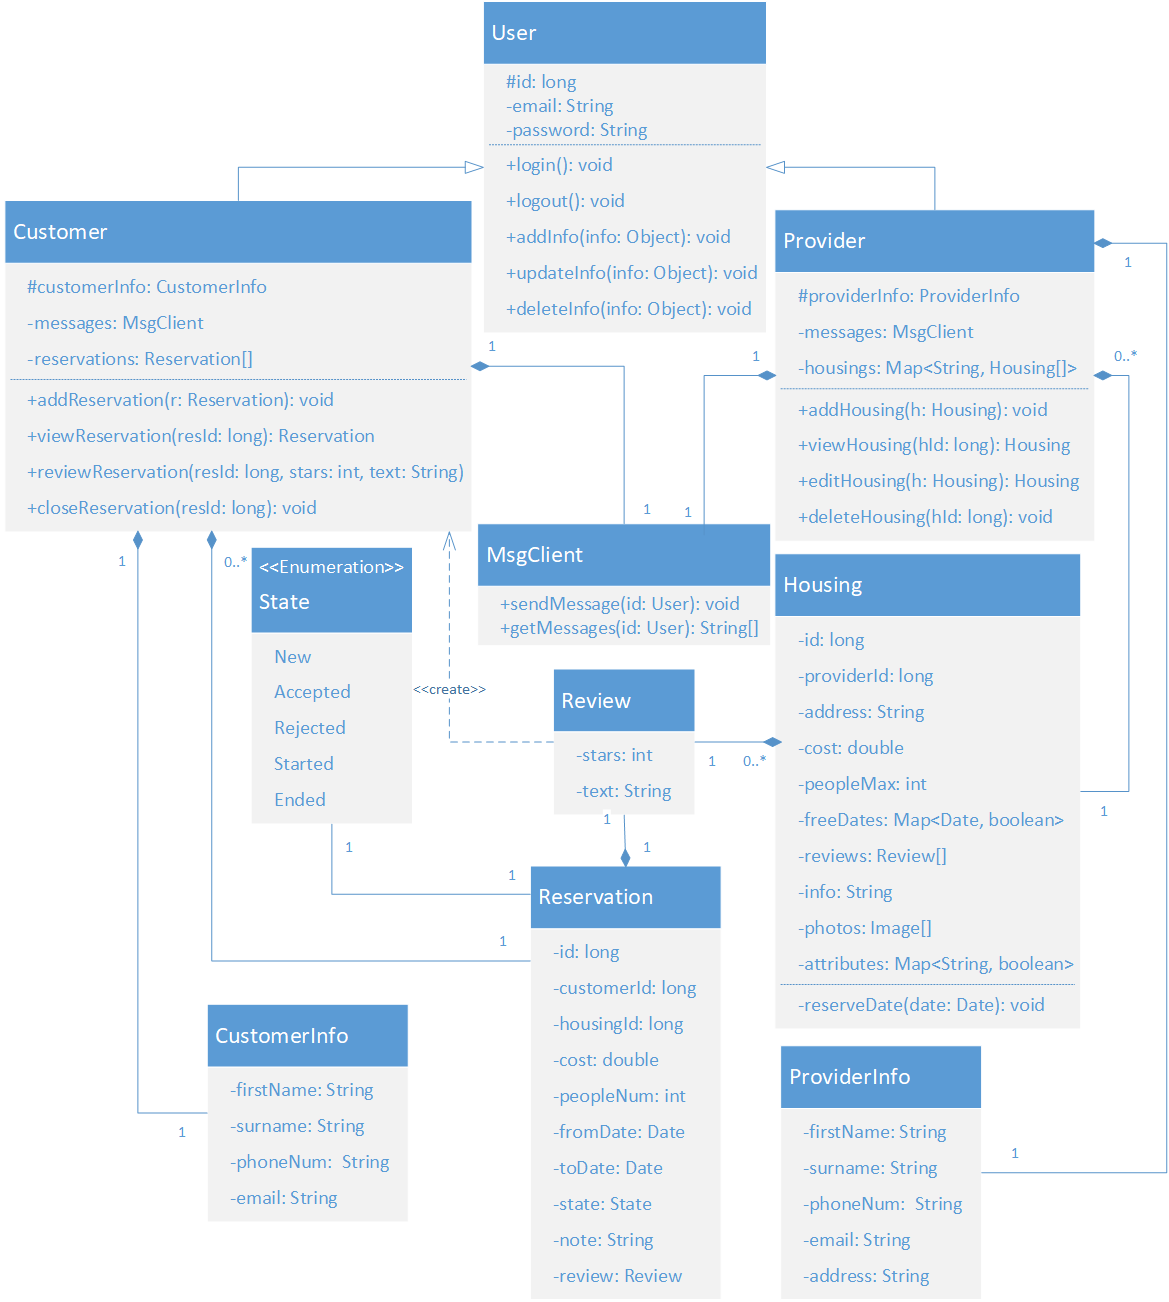
\includegraphics[width=\linewidth]{img/class_diagram.png}
    \caption{Class diagram}
    \label{class_diagram}
\end{figure}

\subsection{Diagramy aktivít a sekvenčné diagramy}
K vybraným netriviálnym prípadom použitia nakreslite
diagramy graficky popisujúce tieto prípady použitia. Nakreslite 2 sekvenčné diagramy a 2
diagramy aktivít.

\subsection{Stavový diagram}
Nakreslite stavový diagram pre vami vyvíjaný systém a v tabuľkách popíšte
jednotlivé stavy a prechody. Môžete vytvoriť aj viacero menších stavových diagramov namiesto
jedného veľkého.

%%%%%%%%%%%%%%%%%%%%%%%%%%%%%%%%%%%%%%%%%%%%%%%%%%%%%%%%%%%%%%%%%%%%%%%%

\section{Akceptačné testy}
Vytvorte testy, na základe ktorých sa rozhodne o tom, či vytvorený systém spĺňa alebo nespĺňa
požiadavky – teda či ho zákazník akceptuje alebo nie. Každý test by mal v tabuľke obsahovať minimálne
tieto časti:
• identifikátor
• prípad použitia, ku ktorému test prislúcha
• cieľ testu (čo overujeme – nanajvýš stručne)
• vstupné podmienky
• výstupné podmienky
• jednotlivé kroky testu
Kroky testu reprezentujú sekvenciu testovania a ku každému kroku prislúcha a je v teste popísaná určitá
akcia (podnet od aktéra) a určitá reakcia systému na tento podnet. Aby bol výsledný systém zákazníkom
akceptovaný, musí splniť všetky testy. Keďže v tomto zadaní systém neprogramujeme ale len
navrhujeme, jednotlivé očakávané reakcie je potrebné si vymyslieť.
Do dokumentácie doplňte aspoň 5 akceptačných testov
• štyri, ktoré súvisia s funkcionálnymi požiadavkami a
• jeden, ktorý overuje nefunkcionálne požiadavky.
PRÍKLAD: \href{https://uim.fei.stuba.sk/wp-content/uploads/2022/10/AkceptacneTestyPriklad.pdf}{AkceptacneTestyPriklad.pdf}

%%%%%%%%%%%%%%%%%%%%%%%%%%%%%%%%%%%%%%%%%%%%%%%%%%%%%%%%%%%%%%%%%%%%%%%%

\section{Projektové plánovanie}
Vytvorte plán tvorby (realizácie) vášho systému.
1. Rozdeľte prácu na aspoň 10 úloh a rozdeľte úlohy pre aspoň 4 ľudí tvoriacich váš tím. Počet si zvoľte
podľa náročnosti témy, ale minimálne musí mať váš tím aspoň 4 členov.
2. Odhadnite časovú náročnosť úloh, naplánujte postupnosť úloh do kalendára.
3. V dokumente v kapitole 4.1 zobrazte Ganttov graf aj s tabuľkou závislostí a postupnosti vykonávania
úloh, s míľnikmi a s WBS (work breakdown schedule).
4. V dokumente v kapitole 4.2. zobrazte sieťový graf pre postupnosti vykonávania úloh.
Na túto úlohu použite vami zvolený systém na projektový manažment (či už offline, lokálny program
alebo ľubovoľný/dostupný online produkt). Zoznam je napr. na:
\url{http://en.wikipedia.org/wiki/Comparison_of_project-management_software}. Úlohou je oboznámiť sa
so systémom na projektový manažment.
Odporúčame: Microsoft Project, Project Libre alebo google: alternatives to ms project

%%%%%%%%%%%%%%%%%%%%%%%%%%%%%%%%%%%%%%%%%%%%%%%%%%%%%%%%%%%%%%%%%%%%%%%%

% \begin{algorithm}
% \scriptsize
% \begin{algorithmic}
%  \STATE <text>
%  \IF{<condition>} \STATE {<text>} \ELSE \STATE{<text>} \ENDIF
%  \IF{<condition>} \STATE {<text>} \ELSIF{<condition>} \STATE{<text>} \ENDIF
%  \FOR{<condition>} \STATE {<text>} \ENDFOR
%  \FOR{<condition> \TO <condition> } \STATE {<text>} \ENDFOR
%  \FORALL{<condition>} \STATE{<text>} \ENDFOR
%  \WHILE{<condition>} \STATE{<text>} \ENDWHILE
%  \REPEAT \STATE{<text>} \UNTIL{<condition>}
%  \LOOP \STATE{<text>} \ENDLOOP
%  \REQUIRE <text>
%  \ENSURE <text>
%  \RETURN <text>
%  \PRINT <text>
%  \COMMENT{<text>}
%  \AND, \OR, \XOR, \NOT, \TO, \TRUE, \FALSE
% \end{algorithmic}
% \caption{Ukážka príkazov pre algorithmic}  
% \label{alg:preview}  
% \end{algorithm}

% \begin{lstlisting}[
%   caption={Ukážka algoritmu},
%   label={lst:main-c},
%   language=c
% ]
% /* Hello World program */

% #include<stdio.h>

% struct cpu_info {
%     long unsigned utime, ntime, stime, itime;
%     long unsigned iowtime, irqtime, sirqtime;
% };

% main()
% {
%     printf("Hello World");
% }
% \end{lstlisting}